\documentclass[12pt]{article}
\usepackage[margin=1in]{geometry}
\usepackage{amsmath}
\usepackage{amssymb}
\usepackage{amsthm}
\usepackage{mathpartir}
\usepackage{graphicx}

\usepackage{cite}

\newcommand{\fT}{\mathcal{T}}
\newcommand{\R}{\mathbb{R}}
\newcommand{\Rnn}{\mathbb{R}^{\ge 0}}
\newcommand{\otw}{\text{otherwise.}}

\renewcommand{\null}{\texttt{null}}
\newcommand{\pointer}[1]{\ast(#1)}
\newcommand{\mradius}[1]{r_{\text{med}}(#1)}
\newcommand{\lev}[1]{\text{Lev}_{#1}}
\newcommand{\tlist}[1]{\text{List}\quad #1}
\newcommand{\tmap}[2]{\text{Map}\quad #1 \quad #2}
\newcommand{\tail}[1]{#1[1:]}
\newcommand{\head}[1]{#1[0]}

\newtheorem{definition}{Definition}
\theoremstyle{plain}
\newtheorem{example}{Example}

\begin{document}
{\centering \Huge \textbf{A Code Search Engine for Go} \\ 
\vspace{0.5cm}
\Large
Harrison Brewton \\
Advised by Aws Albarghouthi \\ 
April, 2020 \\
\normalsize
\vspace{0.1cm} \textit{``All programming language proofs are by induction''} \vspace{0.1cm} \par
}
Creating indexes to aid search through structured data is a finicky business,
and it is especially hard to make these indexes achieve sub-polynomial search time.
This paper looks into problem of automatically creating an index for arbitrary user defined data types.
It details a procedure for the creation of a metric from data types.
It the shows how to use this metric to create an index that provides $O(\log(n))$ bounded search.
The modularity of this system allowed the creation of module \textit{type2met},
which automatically creates metrics from given types.
We then use this module to create a fast search engine for Go functions based on their signature.
We demonstrate its use on a number of popular Go modules.
We conclude with future work.
\section{Background}
\subsection{Metric}
Metrics provide a sensible definition of distance:
the distance from an object to itself is none,
the distance between and object and another is same in either direction,
and the distance between an object and another is the shortest way to get there.
Because of this, they are often used for searching for the nearest objects to some query.
They've been used for image processing, computational biology, computer vision, mealody search, amongst others \cite{chen}.

\subsection{Code Search}
Code reuse has long been the dream of tool designers.
It allows engineers to collectively work on performance, security, robustness, and further reuse.
One part of code reuse is being able to search through a large code base and find functions that have already written.
Previous work \cite{cox} has looked as using raw source code.
Other work \cite{mitchell:hoogle_16_may_2011} has instead used an adhoc rewriting scheme to find the difference between pieces of code,
requiring linear time to search through the code.
\subsection{Implementation and Evaluation}
We have implemented our Type2Metric and Axe in Go.
Type2Metric allows users to use normal structures defined in Go to define their data objects, 
built in Go annotations to provide numeric adjustments in the conversion, 
and a single function call to automatically create metrics that operate over all non-function types in Golang.
We evaluate this converter by its ability to be used in a real world search situation.
We use Type2Metric to automatically create a metric between Go type signatures themselves,
these signatures are parsed out of Go code using Go build tools.
This metric is then used to guide Axe to organize fragments of Go code.
We evaluate Axe by creating indexes over all of the packages in the Go standard library,
and performing random queries on this data.w
\subsection{Contributions}
Our contributions are 

\begin{itemize}
    \item \textbf{The Metric Definition Problem: }
    We describe a novel problem of automatically creating metrics for arbitrary data
    with solutions applicable to search, machine learning, and program synthesis.
    \item \textbf{Automatic Metric Creation: }
    We describe a solution to the previous problem that uses vanilla type objects
    to guide in the automatic creation of a metric for product, sum, list, map, channel, and primitive types.
    \item \textbf{Application: }
    We apply this metric to speed up code search.
    \item \textbf{Evaluation: }
    We give a discussion of our implementation and show the improvements that can be gained through using 
    a metric to improve complex data search.
\end{itemize}
\section{Example}
In this section we present an example of creating a metric from a data type.
\subsection{Example}
Suppose we want to measure how similar two pieces of code are.
Suppose we limit ourselves to the following language, with an obvious interpreation.

\begin{align*}
\text{exp} \to& \text{exp}\quad \text{biop} \quad \text{exp} | \text{singop} \quad \text{exp} | \text{variable} \\
\text{biop} \to & ``+'' | ``*'' \\ 
\text{singop} \to& ``-'' | ``\cos'' | ``\sin''
\end{align*}

There are many ways to do that we might do this,
we might try to just use a simple edit distance
or we might might try to train from a corpus of expressions.
Edit distance requires that we treat our expressions as just linear strings of chracters.
The second option requires us to measure dependent on occurance which is never exactly what we want to measure by.

One place we can start is with the two sets of terminal objects: biop and singop.
Within each class we can use a discrete metric to measure similarity.
That is if the two objects are different we simply say they are some fixed $\kappa$ apart.
This seems as good as anything, though we might want to say that $\cos$ and $\sin$ are somewhat more related, so we give them a $\frac{1}{2}\kappa$ distance.
This is somewhat arbitrarym but seens fine.

We could do a similar approach with variables, but we don't want to say that $counterVariable$ and $countrVariable$ are further apart than any two other words,
and we do not want to give a specific distance for every two words, so instead we can use some edit distance that measures how close the words themselves are.

For the two productions that use exp recursively, we can use the above approaches inductively to find distance between two members of the language that at the top are one of these expressions.
Here's how: first find the distance between left node of the two members, then the right, then the operator used, and then we can simply use a linear combination of these distances to fidn our result.
In this way we can find the distance between any two members of the language.
There is one final question abot what we ought to do if the two words are different at the top level.
For now we will say that we apply a fixed cost ast this often the best approach,
but what we will discuss other options in future sections.

This metric was create through a set of intutions but is not yet something formal.
In the next section we will discuss how to formalize these intutions and others into an algorithm for creating metrics from types.
\section{Type2Metric}
\begin{definition}[Type To Metric Problem]
    Let $\fT$ be some type theory.
    The type to metric problem asks to take some $T \in \fT$,
    and create a metric $d_{T}$.
    $d_{T}$ should satisfy all of the metric properties between any two objects $x$ and $y$ in $T$.
\end{definition}

In the following sections we will use this problem definition to show several solutions to the above problem for different theories.
After seeing these different theories will see how these can be combined to create a complete solution for a reasonably complex type system --
something very similar to Go. 
Specifically, we will look at lists, structs, maps, primatives and we will discuss some extensions for this soultion.
\subsection{Levenshtein Combinator}
Suppose we have two lists $[1, 2, 1, 1]$ and $[1, 3, 2]$.
We want to find the distance between these two lists. 
This is a somewhat ill defined question,
but we can divine a reasonable approach to this question.
We can ask what is the minimum cost to change the first list into the second list.
Cost, for this example, can be defined as the fewest insertions, substitutions, and removals required to convert between the two lists.
There are two things to note here, first different substitutions are more expensive than others,
for example $1000 \mapsto 1$ is definitely more expensive than $2 \mapsto 1$.
For simplicity, we will say a substitution is as expensive as the difference between the two numbers are.
With this in mind we can set a substitution or removal to have some finite cost. Why not $3$?
We choose this number somewhat flippantly, but there is a bit of an art to it.
It's worth noting that this constant sets an upper limit to the substitution cost.
This is because any substitution can be achieved with an insertion and a deletion.
So, in this particular example the substitution between any two numbers is really the minimum of their difference and $6$ (the cost of a deletion followed by an insertion).

The Levenshtein edit distance is a commonly used metric for strings.
It gives the number of substitutions, deletions, or additions to edit one string into another string \cite{wiki:levenshtein}.
It is well known that the normal Levenshtein distance on strings satisfies the properties of a metric.
There are a couple of assumptions that the Levenshtein metric makes:
that all substitutions are of the same cost,
that deletions and additions are of the same cost and the same cost as a substitution.
While this is a safe assumption for strings of characters,
it is not general, as there might be better substitutions than others.
For example, 
it is clear that in a real sense $[1, 2, 3]$ is closer to $[2, 2, 3]$ than it is to $[10, 2, 3]$,
as a $1$ is closer to a $2$ than a $10$;
however, the Levenshtein edit distance would be the same from the first string to the second string (1).
To that end we define the Levenshtein Combinator.

\begin{definition}[Levenshtein Combinator]
Assume that $d : (T \times T) \to \Rnn$ is a metric.
Suppose further that $\kappa$ is any positive real.
Then we say the Levenshtein Combinator of $d$ is  $\lev{d} : (\tlist{T} \times \tlist{T}) \to \Rnn$.
Such that it is defined on lists of $T$.
We define the combinator as: 
$$ \lev{d}(a, b) = \begin{cases} 
    \kappa | \tail{a} | & |b| = 0 \\
    \kappa | \tail{b} | & |a| = 0 \\ 
    \text{min} \begin{cases}
        \lev{d}(\tail{a}, b) + \kappa \\
        \lev{d}(a, \tail{b}) + \kappa \\
        \lev{d}(\tail{a}, \tail{b}) + d(\head{a}, \head{b})  % \lev{d}(\init{a}, b) + \kappa
    \end{cases} & \otw
\end{cases}$$
\end{definition}

The Levenshtein Combinator runs almost the same as the traditional Levenshtein edit distance.
The only differences are the generalizations of the $\kappa$ from 1,
and the addition of the metric between elements of the list.
In fact, the original Levenshtein distance can be recovered by substituting $1$ for $\kappa$,
and the characteristic function $1_{a \neq b}$ as the $d$ metric.
We will now show that the Levenshtein combinator of a metric is itself a metric. 

Identity of indiscernibles and symmetry are pretty obvious, and so are omitted.
The triangle inequality also follows in a similar manner as the proof of traditional Levenshtein \cite{j2kun_2014}.
We first make a simple optimality argument of the Levenshtein distance,
arguing that if there were a shorter distance between two strings it would have been found.
Suppose we are considering a transformation between lists $X$ and $Z$,
that is a series of insertion, deletions, and substitutions.
A transformation from $X$ to some $Y$ followed by a transformation from $X$ to some $Z$
is a transformation from $X$ to $Z$.
As the transformation from $X$ to $Z$ is the minimal transformation,
it follows $d(X, Z) \le d(X, Y) + d(Y, Z)$.
For more detail on this proof see \cite{wiki:levenshtein}.
\subsection{Linear Combinator}
We may want to use multiple definitions of distance between some object.
A simple example is finding the taxi cab distance between two points.
Which is the sum of the distances between two points along any finite number of axes.
We may also want to weigh different distances different values.
This is reasonable if we consider the taxi cab analogy where blcoks might be longer north-south 
than they are east-west.
We can apply this idea generally to any product type,
where we want to define the metric of that type as a linear combination of the metrics of each of the fields.

We will now briefly show that the linear combination of metrics is a metric.
Suppose we have a possible metric $d(a, b) = \sum c_id_i(a, b)$, 
where $c_i$ is a positive real number, and $d_i$ is a metric.
Symmetry follows clearly.
Identity of indescernables follows as each term goes to zero, leaving the sum at zero.
The triangle ineqaulity follows $d(a, b) = \sum c_id_i(a, b) \le \sum c_id_i(a, c)+c_id_i(a, b) = d(a, c) + d(b, c)$.
Thus, we can safely take a linear combination of metrics and arrive still at a metric.
\subsection{Alteration}
Sum types appear rather often.
As a simple example, consider an option type where a value might be present and have some value 
or might not be present and thus have no value.
How might we define a metric for two objects of this type?
Well if both of the objects have values present, then we can simply use the metric for their values (assuming they exist).
If neither exist, then the two objects are exactly the same, and so should have zero distance.
However, what do we do if one exists and the other does not.
One option, and the one taken here, is to simply give them some fixed value.
This choice is clean, but does pin us in a bit.
Consider what happens if the distance between two present values is greater than twice this constant.
We would have broken our metric definition by allowing a shorter route from the first object through an objects of a different type in the alteration
back to the second than the given route between the two objects.
So we revise earlier, and say that the distance between objects of the same type in the alternation is the min of their types metric result 
and the change type constant. 
We formalize this below.

Suppose that we have a tuple $(n, v)$, where $n$ is some natural number less than some $N$,
and a mapping $f : n \to (v \times v \to \R)$.
Then we can define the alteration combinator on these tuples.

\begin{definition}[Alteration Combinator]
Let $T = E \times V$, such that $E$ is some finite set of objects, and $V$ is any other set of objects.
Let $f : E \to (V \times V \to \R)$ be a relation, such that for all $e$ in $E$, 
we have $(f e)$ restricted to $\{ (d, v) \in T : d = e \}$ is a metric on that restriction.
Furthermore, let $\kappa \in \R^{+}$.
Then we define the alteration combinator $Alt : f \to T \times T \to \Rnn$
$$ Alt(f, ((e_1, v_1), (e_2, v_2))) = \begin{cases}
    \min( [f e_1](v_1, v_2), \kappa) & e_1 = e_2 \\ 
    \kappa & \otw
\end{cases}$$
\end{definition}

Symmetry, and identity of indiscernibles is pretty straightforward.
The triangle inequality for $Alt(f)$, is a little trickier.
We consider four cases. 
Let $A$, $B$, and $C$ all be in $E$.
We can consider the triangle inequality as triple of three of these types,
and ask where it will hold. 
If all three are of the same type $(A, A, A)$, then the inequality is inherited by that of $(f A)$.
Consider $(A, A, B)$, then the inequality can be seen $(f A)(A, A) \le \kappa \le (f A)(A, A) + \kappa \le (f A)(A, A) + Alt(f)(A, B)$
Consider $(A, B, B)$, then the inequality can be seen $(f A)(A, B) = \kappa \le \kappa + (f B)(B, B)$.
Consider $(A, B, C)$, then the inequality obviously holds.

\subsection{From Types To Metrics}
\newcommand{\const}{\text{const }}
\newcommand{\sortp}[1]{\text{sortedPairs}(x)}

In Figure \ref{rules} we provide a formalization of rules for generating a metric from a type.
They are largely the same as discussed in the previous subsections, but they have two additions which are worht noting.
First, we haved added maps, a common language type. 
Largely, these are treated like lists;
however to do so we first have to convert them to lists of sorted pairs of keys and values and then we sort them by their key element.
At this point we simply plug them into the levenshtein distance.
Second, we have added pointers.
These just behave as wrappers of their types.
While we are able to prevent some types of pointer cycles by testing if pointers are equal,
this will not terminate for all objects such as two linked lists with one element missing.
More work needs to be done to resolve this.

There is a cheap proof that needs to be made where we show that all of the distance fucntions created here are in fact metrics.
As a base case, it is clear that numbers are metrics.
We have sufficiently shown that all other combinations are metrics in the previous.
So, by induction these are all metrics.
We have implemented these rules in a tool called type to metric which we will discuss later.

\begin{figure}
\begin{mathpar}
\inferrule*[Right=Lists]{\Gamma \vdash x, y : \tlist{T}}
    {d(x, y) = \lev{T}(x, y)} 
\\
\inferrule*[Right=Products]{\Gamma \vdash x, y :  (T_1, T_2, \ldots, T_n) \\ \Gamma \vdash c_i = \const((T_1, T_2, \ldots, T_n))}
    {d(x, y) = \sum_{i=0}^n c_id_{T_i}(x_i, y_i)}
\\
\inferrule*[Right=Sums]{\Gamma \vdash x, y : T_1 | T_2 | \ldots | T_n \\ 
    \Gamma \vdash \kappa = \const((T_1 | T_2 | \ldots | T_n))}
    {d(x, y) = 1_{\text{type}(x) = \text{type}(y)} \min(\kappa, d_{\text{type}(x)}(x, y)) + 
    {1_{\text{type}(x) \neq \text{type}(y)}\kappa}}
\\
\inferrule*[Right=Map]{\Gamma \vdash x, y : \tmap{T_1}{T_2}}{d(x, y) = \lev{T}(\sortp{x}, \sortp{y})}
\\ 
\inferrule*[Right=SameAddressPointer]{\Gamma \vdash x, y : \pointer{T}, x = y}
{d(x, y) = 0}
\\ 
\inferrule*[Right=DifferentAddressPointer]{\Gamma \vdash x, y : \pointer{T}, x \neq y}
{d(x, y) = d_T(\pointer{x}, \pointer{y})}
\\ 
\inferrule*[Right=Number]{\Gamma \vdash x, y: T \\ \Gamma T <: \text{Number}}{d(x, y) = |y-x|}
\end{mathpar}
\caption{Rules for converting types to metrics}
\label{rules}
\end{figure}
\subsection{Some Additions}
\subsubsection{Recursive Type Promotion}
\section{Example: Go Code Look Up}
\subsection{Generics}
\section{Metric Trees}
\input{metricTrees.tex}
\section{Implementation}
We implemented the automatic type to metric converter,
vantage point tree,
and Go type extractor in Go\cite{github}.
We seek to answer the following two research questions:
\begin{itemize}
    \item[\textbf{RQ1}] Can we automatically create metrics from given types?
    \item[\textbf{RQ2}] Are these metrics effective in reducing time complexity of problems?
    \item[\textbf{RQ3}] Do we get adequate results from our query to axe?
\end{itemize}
\section{Evaluate}
Here \ref{dist1plot} \ref{dist6plot}
\begin{figure}
    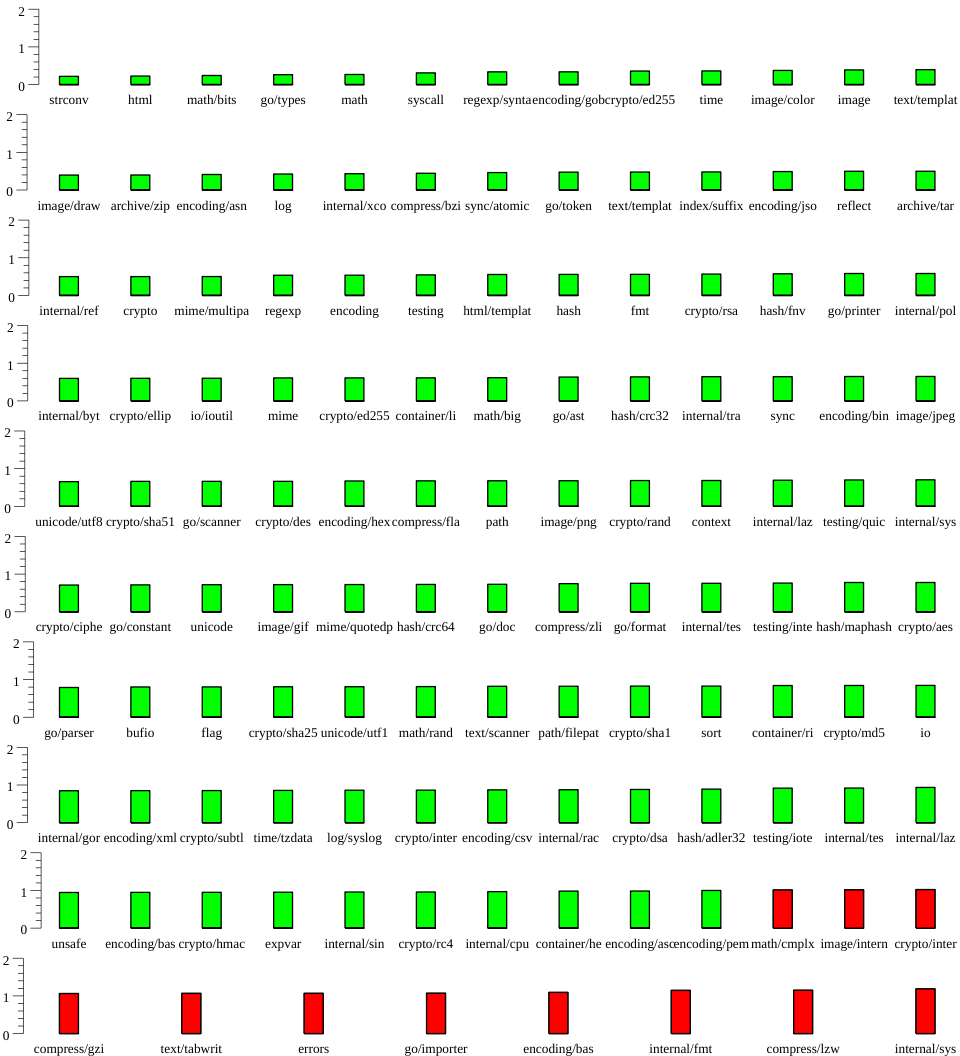
\includegraphics[width=\textwidth]{example1.png}
    \label{dist1plot}
    \centering
    \caption{Each Go module was indexed and then randomly queried.
    Speed up over linear search for a search distance of $1$ is plotted for each Go module.
    Green idicates search was fater, red otherwise.}
\end{figure}
\begin{figure}
    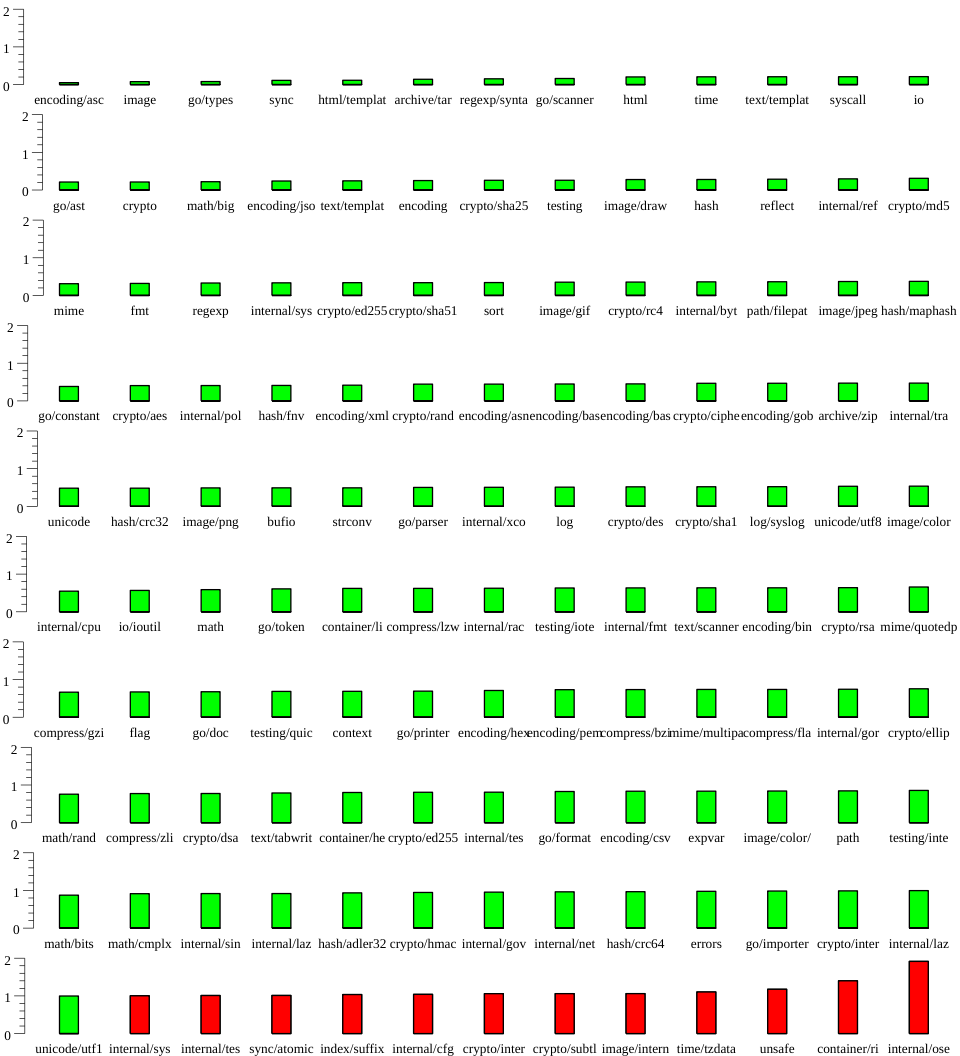
\includegraphics[width=\textwidth]{example6.png}
    \label{dist6plot}
    \centering
    \caption{Each Go module was indexed and then randomly queried.
    Speed up over linear search for a search distance of $6$ is plotted for each Go module.
    Green idicates search was fater, red otherwise.}
\end{figure}
\section{Related Work}
\subsection{Type Based Search}
Using types for search has been an idea for a long time \cite{ReusablePolyType,TypeAsKey},
though these early methods often went through the process of doing a full unification and only returning those functions which perfectly unify with the query.
Hoogle \cite{hoogle} is a widely used search engine for Haskell functions.
For a while it used this pure unification strategy.
Sincer version 5, it has moved to ad-hoc search.
It essentially does random edits on the query, each edit with a particular cost,
and it then lists types based on the number of edits required to move from type to another type.
This was a large improvement in query quality over previous results as it allows users to enter imperfect types.
However, because it uses this adhoc approach it still requires linear time to the search.
\subsection{Google Code searchSearch}
Google code search was a popular code search engine that allowed individuals to search for code for reuse \cite{codeSearch}.
It was designed to be language agnostic, and as opposed to type based search would just use the plain text of code's source.
It used an inverted look up table that would search based on various trigrams that appeared in a querier's search \cite{cox}.
Using this trigram method is was able to achieve a strong index complexity;
however, it did not take advantage of structural language features such as type signatures.
\subsection{2Vec's}
The ``2vec'' genre is a common genre of paper in the machine learning community \cite{mikolov2013distributed,jaeger2018mol2vec}.
The general idea is to take some object such as string, molecule, or whole graph and convert those objects into a vector.
These vectors are then used in various machine learning tasks such as translation and classification.
This is done using domain specific knowledge about the type being converted into a vector.
Type2Metric provides a somewhat similar feature, but only converts to metrics. 
These metrics can be used for many tasks but can not yet be put into a machine learning model,
though a machine learning model could be applied to the constants used by Type2Metric.
\section{Future Work: Best Approximation}
One natural extension of this work is create a best approximation of types in some euclidean space.
The idea would be to find a way to embed the points of the metric space in some arbitrary euclidean space chosen 
by using the metric of the metric space to try to space out instantces of a type.
This presents its own problems particularly because the points of the metric spaces we have been dealing with 
deal with arbitrarly large trees of data.
However, if we ware able to approximate this embedding,
then we can convert arbitrary datastructures into reasonable fixed dimension vectors.
\section{Conclusion}
We presented the problem of generating metrics based on a type.
We then provided a reasonable solution to this problem,
the first know to the author.
We then implemented this solution in a tool called Type2Metric,
which takes a type defined in GoLang and creates a metric from that type.
We then made an instance of this conversion,
using Type2Metric,
that takes Go type signatures and creates a metrizable object.
We then used this this metric to create a Go Search tool called Axe,
which is the first $O(log(n))$ type based search tool known to the author.

\bibliographystyle{unsrt}
\bibliography{biblio}
\end{document}